\begin{frame}
    \frametitle{Dynamic traffic assingment - Problem}
    \begin{columns}
      \begin{column}{0.5\textwidth}
        \begin{figure}
          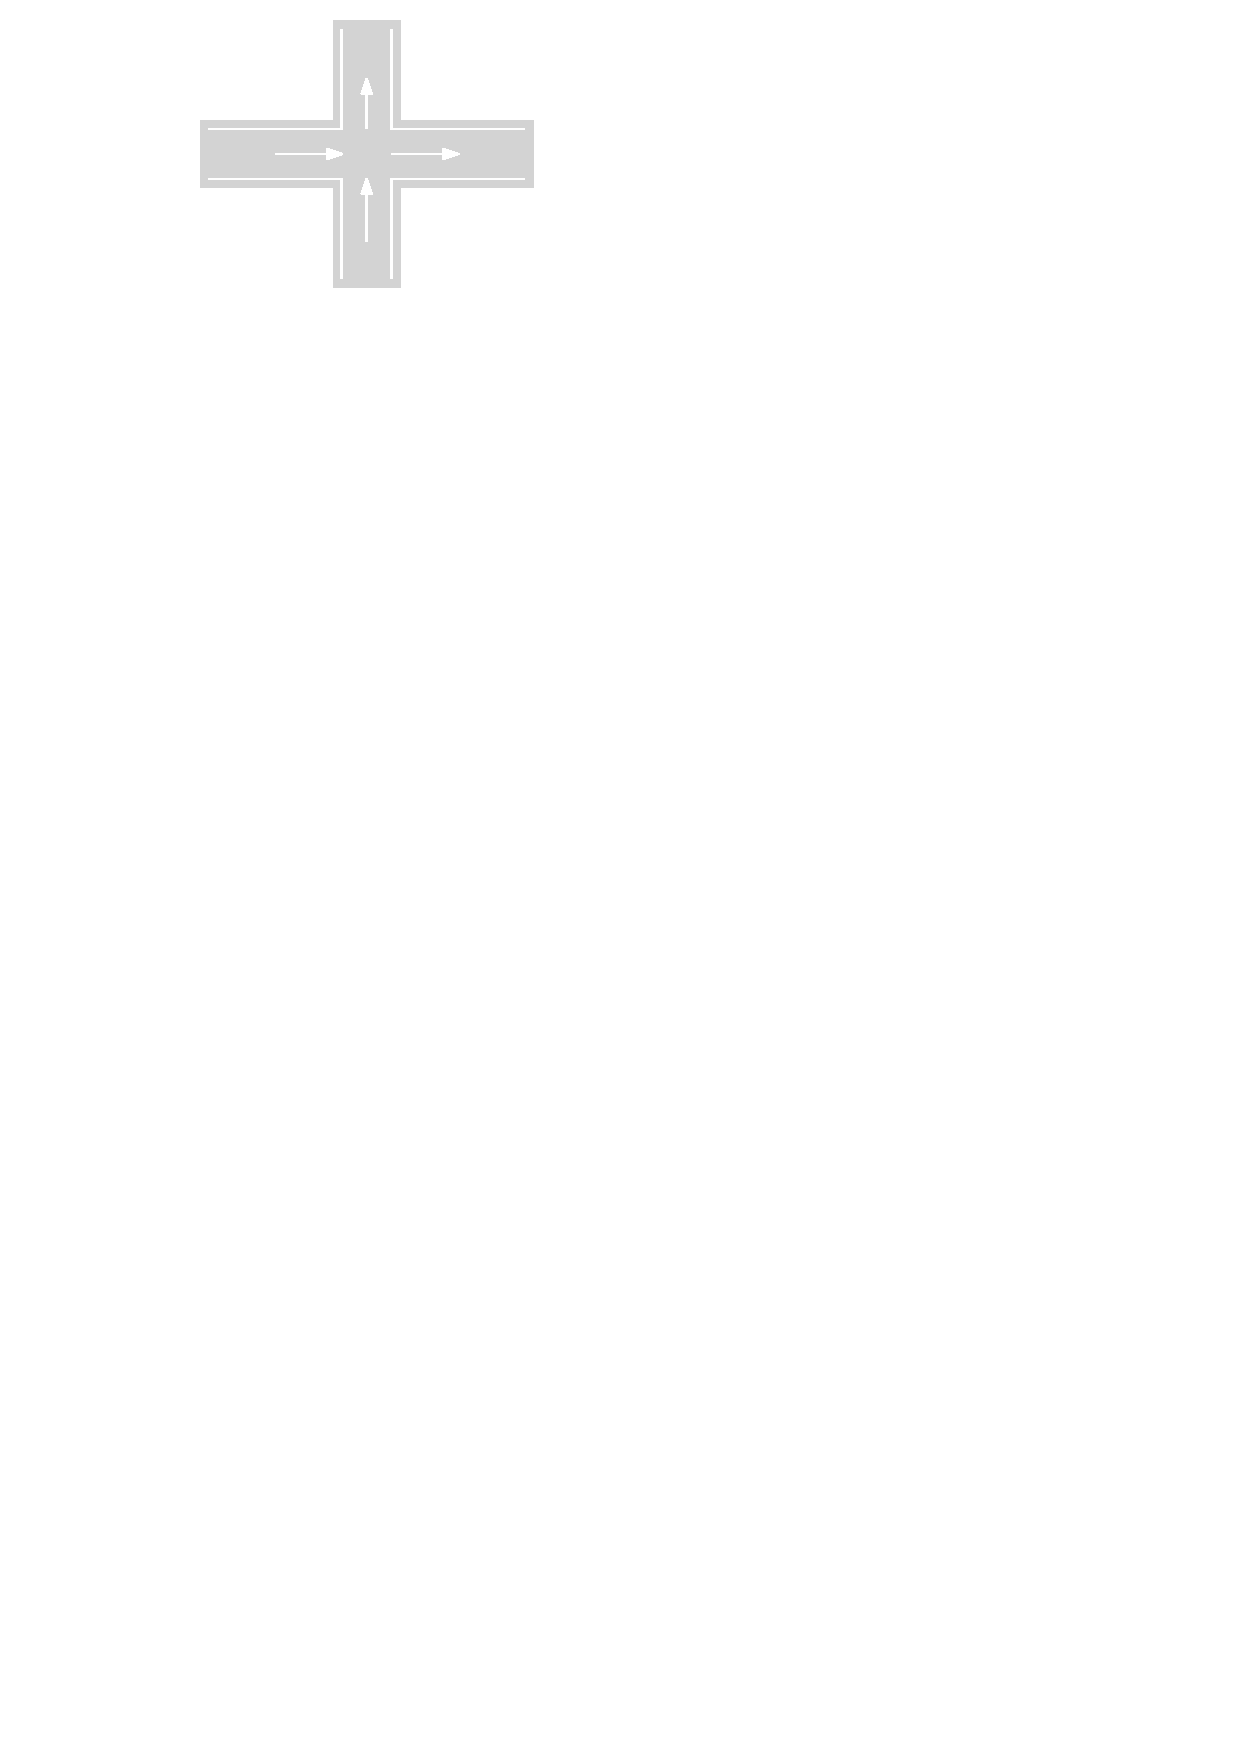
\includegraphics[width=0.8\linewidth]{fig_22_intersection}
        \end{figure}
      \end{column}
      \begin{column}{0.5\textwidth}
        \begin{block}{Questions}
          How to assign the flow at time \(t\)?
        \end{block}
        Some key principles\footcite{Coclite:2005}: 
        \begin{enumerate}
          \item Flow conservation 
          \item Flow maximization
          \item Infrastructure limitations
          \item Set/calibrate drivers' preferences
        \end{enumerate}
      \end{column}
    \end{columns}
    Unless the drivers preferences are well known the solution to the DTA problem is undetermined. 
\end{frame}